\chapter{Adapting a Meta-Model to the Pivot Model}
\label{chapter:pivotModelAdaptation}

\begin{flushright}
\textit{Chapter written by Michael Thiele}
\end{flushright}

DresdenOCL is built to work with different meta-models / \acs{DSL}s. In order to
use new meta-models one has to create an adapter plug-in that adapts the
meta-model to the pivot model of the toolkit. To ease this process, DresdenOCL
includes a code generator that creates adapter stubs.



\section{The Adapter Code generation}

The code generator is located in the plug-in 
\reference{tudresden.ocl20.pivot.codegen.adapter}. The only prerequisites are 
the core features (\reference{tudresden.ocl20.feature.core}) of DresdenOCL and
the meta-model to adapt that has to be modeled in \acs{EMF} Ecore.

In the following Ecore itself will be adapted to the pivot model (this has been 
done already for DresdenOCL, but serves the purpose of showing the adaption
mechanism on a well known meta-model). 
Figure~\ref{pic:pivotModelAdaptation:EcoreOverview} shows the Eclipse standard 
editor for Ecore models with the Ecore model opened. Since the adaptation of 
different repositories is allowed, one has to specify the resource from which a 
model can be loaded. This can be done via an annotation as shown in 
Figure~\ref{pic:pivotModelAdaption:CreateAnnotation}. In the \eclipse{Properties
View} enter \code{http://www.tu-dresden.de/ocl20/pivot/2007/pivot\-model} as 
\code{Source} (see Figure~\ref{pic:pivotModelAdaption:AnnotationProperties}). 
Create a new details entry for the annotation 
(Figure~\ref{pic:pivotModelAdaption:CreateAnnotationDetails}) and enter 
\code{Resource} as \code{Key} and \code{org.eclipse.emf.ecore.resource.Resource}
as \code{Value} (see 
Figure~\ref{pic:pivotModelAdaption:AnnotationDetailsProperties}).

\begin{figure}[!p]
	\centering
	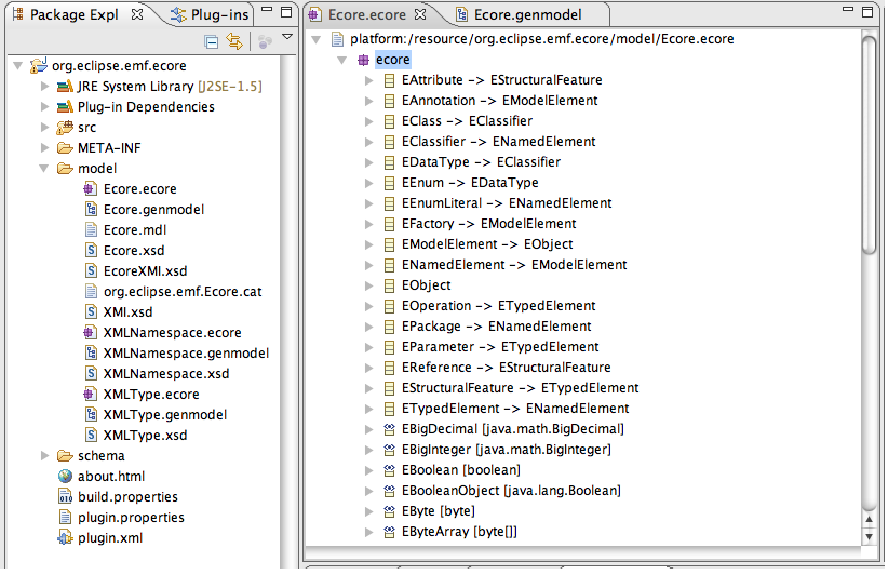
\includegraphics[width=1.0\linewidth]{figures/pivotModelAdaption/EcoreOverview}
	\caption{The Ecore model opened in Eclipse.}
	\label{pic:pivotModelAdaptation:EcoreOverview}

  \vspace{3.0em}
  
	\centering
	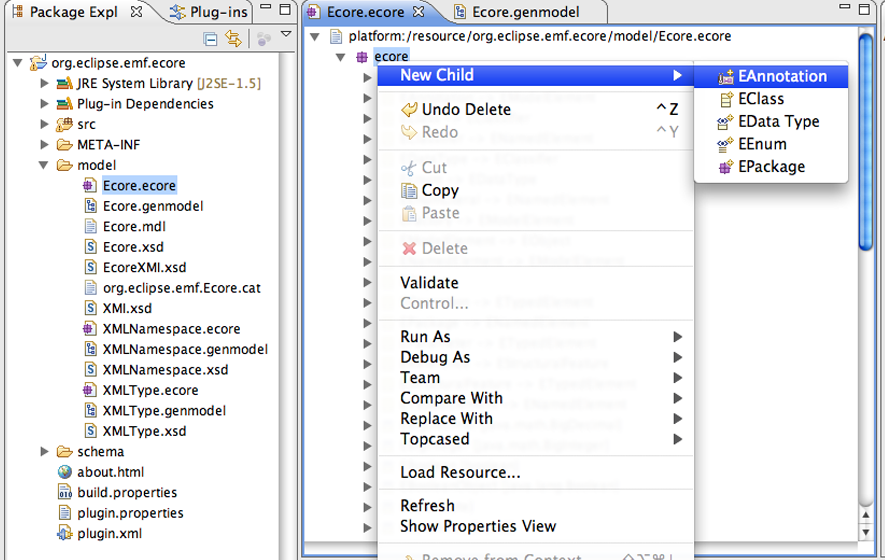
\includegraphics[width=1.0\linewidth]{figures/pivotModelAdaption/CreateAnnotation}
	\caption{Create an annotation for the Ecore package.}
	\label{pic:pivotModelAdaption:CreateAnnotation}
\end{figure}

\begin{figure}[!p]
	\centering
	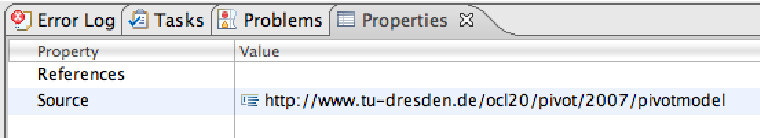
\includegraphics[width=0.8\linewidth]{figures/pivotModelAdaption/AnnotationProperties}
	\caption{The Properties View for the annotation.}
	\label{pic:pivotModelAdaption:AnnotationProperties}

  \vspace{5.0em}
 
 	\centering
	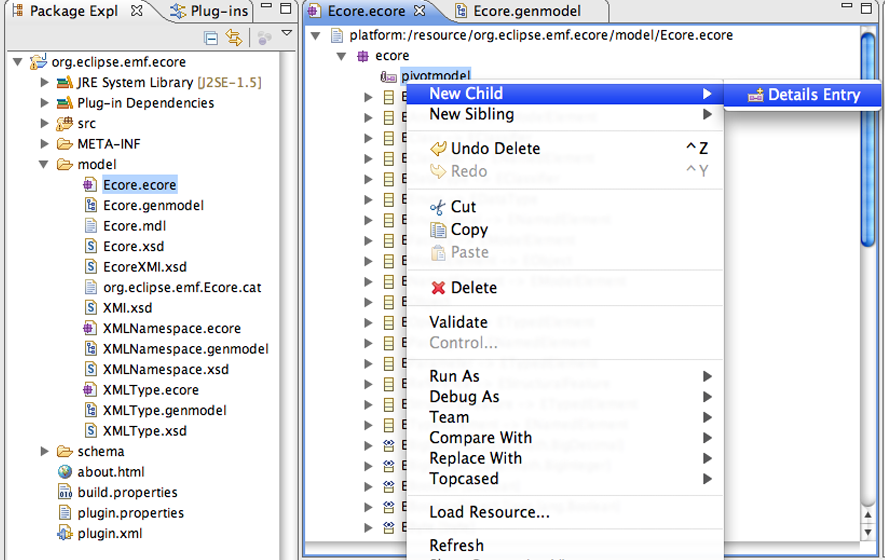
\includegraphics[width=1.0\linewidth]{figures/pivotModelAdaption/CreateAnnotationDetails}
	\caption{Create annotation details for the annotation.}
	\label{pic:pivotModelAdaption:CreateAnnotationDetails}

  \vspace{5.0em}
 
 	\centering
	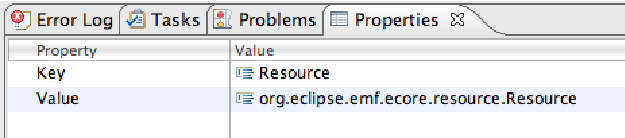
\includegraphics[width=0.8\linewidth]{figures/pivotModelAdaption/AnnotationDetailsProperties}
	\caption{The Properties View for the annotation details.}
	\label{pic:pivotModelAdaption:AnnotationDetailsProperties}
\end{figure}

To adapt types of the meta-model to the pivot model, choose the type to adapt
and create a new annotation (similar to resource) and a corresponding details 
entry with \code{PivotModel} as \code{Key} and the specific pivot model type
name as \code{Value}. In Figure~\ref{pic:pivotModelAdaption:EClassAnnotation}
the meta-element \model{EClass} is adapted to the pivot model type \model{Type}.
This step has to be repeated for every meta-model type that can be adapted to
the pivot model. In this example this would be:

\begin{itemize}
  \item \model{EClass} --\textgreater \model{Type}
  \item \model{EDataType} --\textgreater \model{PrimitiveType}
  \item \model{EEnum} --\textgreater \model{Enumeration}
  \item \model{EEnumLiteral} --\textgreater \model{EnumerationLiteral}
  \item \model{EOperation} --\textgreater \model{Operation}
  \item \model{EPackage} --\textgreater \model{Namespace}
  \item \model{EParameter} --\textgreater \model{Parameter}
  \item \model{EStructuralFeature} --\textgreater \model{Property}
\end{itemize}

When finished, switch to the \keyword{Generator Model} (see 
Figure~\ref{pic:pivotModelAdaption:EcoreGenModel}). Open the context menu on 
the root element and choose \code{Generate Pivot Model adapters} like shown in
Figure~\ref{pic:pivotModelAdaption:GeneratePivotModelAdapters}. A new plug-in 
is created. It is named after the conventions of the DresdenOCL:
\code{tudresden.ocl20\linebreak[0].pi\-vot\linebreak[0].meta\-mo\-dels.<meta-model name>}. The package explorer is shown in Figure \ref{pic:pivotModelAdaption:GeneratedPlugin}.

Every created class marked blue 
(\url{http://www.eclipse.org/modeling/emft/?project=mint/}) has methods with an
\code{@generated} annotation. The locations where to alter the generated code 
are also marked with \code{TODO}s. After replacing the \code{TODO}s with real 
code, the adapter is complete and can be used together with the DresdenOCL.

\begin{figure}[!b]
	\centering
	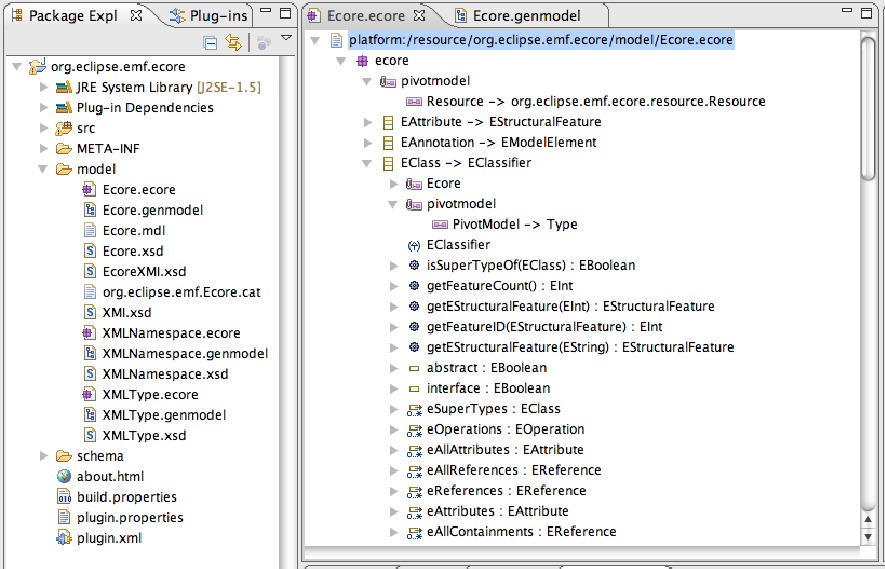
\includegraphics[width=1.0\linewidth]{figures/pivotModelAdaption/EClassAnnotation}
	\caption{The EClass annotation.}
	\label{pic:pivotModelAdaption:EClassAnnotation}
\end{figure}

\begin{figure}[!p]
	\centering
	\includegraphics[width=1.0\linewidth]{figures/pivotModelAdaption/EcoreGenModel}
	\caption{The genmodel of the Ecore model.}
	\label{pic:pivotModelAdaption:EcoreGenModel}

  \vspace{4.0em}
  
  \centering
	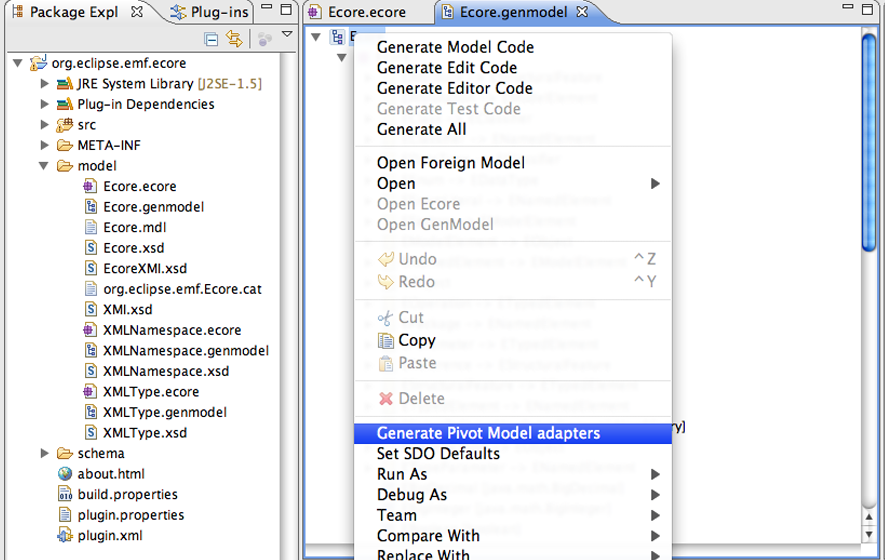
\includegraphics[width=1.0\linewidth]{figures/pivotModelAdaption/GeneratePivotModelAdapters}
	\caption{Right-click on Ecore and select 'Generate Pivot Model adapters'.}
	\label{pic:pivotModelAdaption:GeneratePivotModelAdapters}
\end{figure}

\begin{figure}[!htbp]
	\centering
	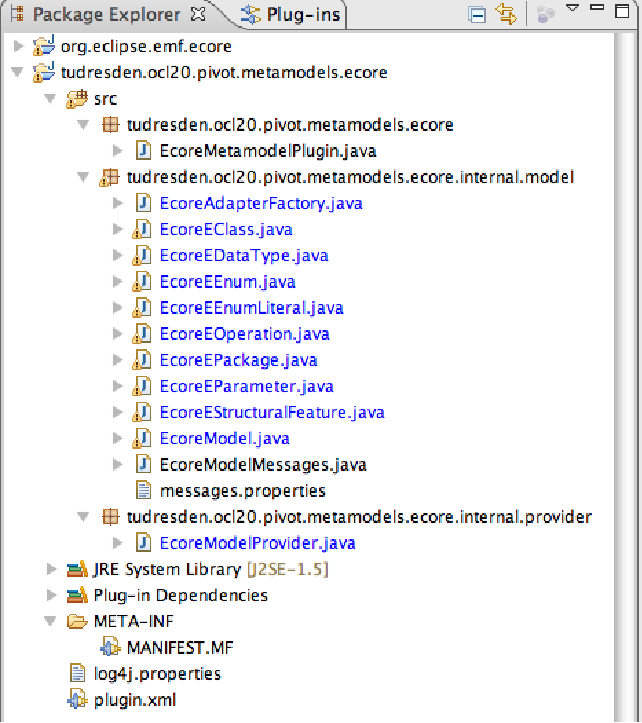
\includegraphics[width=0.7\linewidth]{figures/pivotModelAdaption/GeneratedPlugin}
	\caption{The structure of the generated plug-in.}
	\label{pic:pivotModelAdaption:GeneratedPlugin}
\end{figure}



\section{Summary}

This chapter explained, how an annotated Ecore model can be used to generate 
adapter stubs for a meta-model that shall be adapted to the pivot model of
DresdenOCL. For further implementation details investigate the source code of
the existing adapted meta-models, such as Java, \acs{UML} and Ecore. To test 
the new adapter, read Chapter~\ref{chapter:metaModelTestSuite} that introduces 
the \keyword{Generic Meta-Model Test Suite} that allows test-driven development 
of the adapter code.
